\begin{artengenv}{Radosław Kycia}
	{Information and brain}
	{Information and brain}
	{Information and brain}
	{Masaryk University, Department of Mathematics and Statistics\\
	Cracow University of Technology, Faculty of Computer Science and Telecommunications\label{kycia_anfang}}
	{We present the consequences of the assumption of the classical and quantum nature of information storing and processing in the brain. These assumptions result in different behaviours of consciousness under a hypothetical brain copy experiment. The subject is important in the context of `mind uploading' considerations.}
	{classical information, quantum information, brain models, mind uploading.}
	
	


%%%%%%%%%%%%%%%%%%%%%%%%%%%%%%%%%%%%%%%%%%%%%%%%%%%%%%%%%%%%%%%%%%%%%%%%%%%%
%Introduction
%%%%%%%%%%%%%%%%%%%%%%%%%%%%%%%%%%%%%%%%%%%%%%%%%%%%%%%%%%%%%%%%%%%%%%%%%%%%
\section{Introduction}
%%%%%%%%%%%%%%%%%%%%%%%%%%%%%%%%%%%%%%%%%%%%%%%%%%%%%%%%%%%%%%%%%%%%%%%%%%%%
\lettrine[loversize=0.13,lines=2,lraise=-0.03,nindent=0em,findent=0.2pt]%
{T}{}he brain is the most complicated organ in the human body and it is still not well understood. It is responsible for `high-level' capabilities such as reasoning and intelligence. Recently, greater efforts have been made to understand the structure and its exact working principles through the Brain Research through Advancing Innovative Neurotechnologies (BRAIN) project, announced by the United States Government in 2013 \parencite{BRAINInitiative}. This project mainly focuses on the structural approach to the brain and on collecting data on the neuronal activities within it.

Currently, there exist exact simulations of the brain parts up to the level of cells, e.g. the Blue Brain Project \parencite{BlueBrainProject}. There are also mathematical models of some of its regions, e.g. the hierarchical temporal memory (HTM) of the neurocortex \parencite{CortexModel1, CortexModel2} which is based on hidden Bayesian networks \parencite{KurzweilHowToCreateBrain}. These ideas have been used successfully in software for speech and image recognition. There are also interesting connections of models of the visual cortex with differential geometric structures \parencite{VisualCortex}, describing structures above the level of single neurons and their interconnections.

At the level of single cells, there are various models of neurons and their interactions used in computational neuroscience, see e.g. \parencite{ModellingNeurons} and references therein. In short, neurons communicate with other neurons, exchanging electric impulses (modifying ion density locally within the cell or using chemical neurotransmitters at synapses, the interface between neurons). The neuron has some threshold of activation above which it `fires' producing a spike in voltage. In models based on neurons, memory and learning ability of the brain result from a `plasticity' of neuron synapses---change of neurons interaction intensities encode new and modify existing data in the brain. In this approach, the topology of the neural network as well as the properties of single neurons are taken into account. These models use non-linear differential equations, stochastic models, and/or a control theory approach.

However, there is no unifying idea of precisely how the brain works and how elements/parts induce high-level capabilities. There is not even any consensus regarding whether the brain operates on classical principles alone, or whether quantum principles need to be included as well. There are reports on the importance of quantum mechanical processes in neurons  \parencite{EmperorsNewMind, PenroseQuantum1, PenroseQuantum2}. Furthermore, a new discipline of quantum biology \parencite{QuantumBilogy} has been established: the discipline of biology that examines the relevance of quantum level processes (tunneling, entanglement) in living organisms. We want to strongly stress that the current state of knowledge indicates that quantum processes are not essential on scales larger than chemical compounds \parencite{QuantumBilogy}. In our presentation, we do not exclude these as they provide an effective comparison between the classical and quantum approaches to brain functionality. New results suggest that the quantum processes as entanglement is possible also in hight temperatures \parencite{HightTempEntantgelemnt}. The other reason is that we do not know with precision the basic principles according to which the brain as a whole operates, even if the entirely classical paradigm currently appears most probable.


It is currently impossible to describe the brain structure strictly and there are many gaps in the present state of knowledge of brain operating principles. Therefore, in this article we reduce all complex problems to maximally simple and general ones. We consider the possible implications of the assumption that the brain works solely on classical principles and compare it with the quantum level approach. This enables us to define transcendental properties (i.e. if the properties of the brain configuration can be copied beyond the body). We elaborate this by considering a 
\textit{Gedankenexperiment} of brain copy to a virtual model. At the current level of technology and our understanding of the brain it is impossible to make. Such kinds of thought experiments provide a framework for understanding some aspects of consciousness from different angles \parencite{MindUploading2, KurzweilHowToCreateBrain}. This experiment fits into contemporary philosophical considerations regarding mind uploading \parencite{Transhumanizm, MindUploading, MindUploading2}. The other aim is to continue the discussion from \parencite{EmperorsNewMind} on the implications of the assumptions as to the principles according to which the brain operates.

The paper is organized as follows. In the next section, a review of the basic facts and properties of classical and quantum representation of information is provided. The section thereafter contains a formulation of the thought experiments on copying brain functionality to a machine. This allows us to deduce how assumptions regarding quantum or classical information in the brain will result in the possibility of copying the brain and therefore on the uniqueness of `consciousness'. The final section presents our conclusions.



%%%%%%%%%%%%%%%%%%%%%%%%%%%%%%%%%%%%%%%%%%%%%%%%%%%%%%%%%%%%%%%%%%%%%%%%%%%%
\section{Classical and quantum information properties}
%%%%%%%%%%%%%%%%%%%%%%%%%%%%%%%%%%%%%%%%%%%%%%%%%%%%%%%%%%%%%%%%%%%%%%%%%%%%
In this section, we focus on the properties of classical and quantum representation of information and their computation, which will prove useful in the next section.



%%%%%%%%
\subsection{2.1. Classical representation of information}
%%%%%%%%
We start to outline the information theory. It is a large subject including many branches \parencite{RezaInformation}. Here we focus on the basic properties that will be useful in subsequent sections.

Information describes results of our interaction with some object---a source of information. We consider a binary source that can produce two types of experimental outputs when we interact with it by recording answers for questions, e.g., about shape, colour or other information about the object. This set of questions and answers constitutes one way in which we encode our interactions with the world. We can associate these two outputs with letters (usually called `bits' in this context) from the alphabet $A=\{0,1\}$. Therefore, the output of the experiment is a sequence of letters, e.g. a word of length $N$ is an element of $A^N=A\times \ldots \times A$, where $\times$ indicates the Cartesian product. In computer science, the sequence of eight bits constitutes a byte. In binary computers, bits are stored in a physical structure called a `register' that is constructed from cells that are sequentially organized and can store one of two values from $A$. 

The numbers (integer, real, complex, etc.) can be coded into letters of $A$. This procedure starts by associating elements $A$ as representation of numbers of base\footnote{$\#A$ means the number of elements of the set $A$.} $N=\#A$, where letters from $A$ are associated (with some assumed order) to digits $\{0,1,\ldots, N\}$. Then the coding of a real number is a set (possibly infinite) of answers for questions if some number in the decoding procedure is larger than $lN^{n}$, where $n$ is an integer number and $l$ is a number associated with a letter of alphabet. For instance, for binary system $A=\{0,1\}$ we have  $5 = 1\cdot2^{0}+0\cdot 2^{1} + 1\cdot 2^{2} = 101_{2}$, that is, $2^{2} < 5 <2^{3}$ and $ 2^{0} \leq 5-2^{2} < 2^{1}$, which is process of discretization/quatization. There is also an interesting question to be raised about the efficiency of the coding of numbers. The most efficient choice of base is for the base of natural logarithm  $N=e$, see e.g., \parencites{kycia_information_2020}{KyciaNiemczynowicz} and references therein.

Moreover, for an analog signal that is described by a function $f:\mathbb{R}\rightarrow \mathbb{R}$, we can quantize and sample it in specific time intervals. This gives us a discrete representation of the signal. The bound on information loss during this process in the simplest case is controlled by the standard Nyquist--Shannon sampling theorem for equidistant sampling \parencite{Probing, RezaInformation} or by more elaborated sampling theorems.

All the above considerations reinforce the statement that we can restrict ourselves to  $A=\{0,1\}$ as each piece of information can be reduced with arbitrary accuracy to the sequence from $A$, providing a suitable coding method. These data can be processed digitally.

There also exists an approach to information in a statistical sense developed by Shannon \parencite{RezaInformation}. It focuses on analysis statistical properties of subsequences of bits in information. This statistical approach focuses on the efficiency of coding and not on the information itself, because a string of `bits of information' is treated statistically. Therefore, we will not deal with this notion in this paper. We do not care here about the efficiency of coding, as we will try to reduce the problem to fundamental principles, not necessarily efficient ones.


Later, we will be using the copy machine defined by the following operation:
\begin{equation}
\begin{array}{c}
 c: A^N \times A^N \rightarrow A^{2N}, \\
 c(M,a)= [M,M],
\end{array}
\end{equation}
where $a$ is an arbitrary sequence of $N$ bits, and the result is repeated two times the pattern of bits $M \in A^N$. After copying, the linear projection on the second component can be performed to isolate the copied data. Such duplication can be derived from the diagonal morphism  \parencite[see][]{RosettaStone_Baez} $\Delta :A \rightarrow A \times A$ that acts as $\Delta (x) = (x,x)$ for some $x \in A$.

The most important observation is that the copy operation can be conducted without perturbing the physical memory. This results from the statement that classical measurements can be designed not to perturb a memory based on the classical laws of physics. This is aside from the notion of information and is instead a statement on classical physics itself as well as the representation of information in systems obeying classical laws. We will see below that this changes when information is stored in quantum systems: this will be the core of our further considerations.


Information stored in classical system will be called classical information for short. In the next subsection, a review of quantum information properties is presented.

%%%%%%%%
\subsection{2.2. Quantum representation of information}
%%%%%%%%

The natural framework for quantum information/computing is a Hilbert space, i.e. data are represented as vectors of a complex inner product vector space, which is also a complete topological space \parencite{FunctionalAnalysisReed}. In the standard approach, a finite-dimensional vector space is used with a base of dimension $N >0$.

A single quantity of information is stored as a (complex) linear combination of base vectors. Depending on the dimensionality of the base, it is called a `qubit' for $N=2$ and a~`qudit' for $N>2$ \parencite[see e.g.][]{QuantumComputing}. We will focus here on qubits because, for qudits, the description is analogous. The dimension of the space determines the number of elements in the vector base and is called the `degree of freedom' of the qudit. For a qubit, the normalized vector describes a point on a sphere $S^{2}$ called the Bloch sphere \parencite{QuantumComputing}. This point on this sphere can be represented as a set of coordinates and even decoded to, for instance, the binary form described previously. Therefore, we can code classical information in qubits and vice versa. As we will see, the difference is in the physical properties of the quantum carrier of information. 

For quantum states the Hilbert space of the compound system is the tensor product of its constituents, in contrast to the Cartesian product for classical information. Therefore, if $\mathcal{H}$ is a Hilbert space for a single qubit then a register of $r>0$ such qubits is realized as a device that can store elements from
\begin{equation}
 \bigotimes_{k=1}^{r} \mathcal{H}.
\end{equation}

The square of the inner product of two qubits has the interpretation of the probability of finding the state of the system described by the first qubit in the state of the system described by the second qubit. Therefore, its value belongs to the unit interval $[0; 1]$ for all times. This imposes substantial requirements on the type of allowable operations realizing computations on quantum registers, namely they have to be unitary operations, that is, surjective isometries of the inner product.

There are two fundamental `no-go' properties that characterize quantum in formation and that will be used in the following section. They characterize a quantum representation rather than information itself. The first is the no-cloning theorem, which in its elementary version was originally published in \parencite{NoCloning_WootersZurek}. The formulation uses the unitary `copying machine'/cloning operator $U$ which copy states as follows\footnote{The notation $|\psi>$ for a vector in the Hilbert space $\mathcal{H}$ was invented by Paul Adrien Maurice Dirac and is called `bra-ket' notation \parencite{QuantumComputing}.}
\begin{equation}
 \begin{array}{c}
  U: \mathcal{H} \otimes \mathcal{H} \rightarrow \mathcal{H}\otimes \mathcal{H}, \\
  U( | \psi> \otimes |a >) = | \psi> \otimes |\psi >,
 \end{array}
\end{equation}
where $|a>$ is an arbitrary (non-zero) vector in $\mathcal{H}$ onto which copy is made. The no-cloning theorem of Wootters and \.{Z}urek reads
\begin{Theorem}
\label{Th.NoClonning}
 If $dim\mathcal{H}>1$ then no cloning machine exists.
\end{Theorem}

The proof is simple\footnote{
We provide the proof from \parencite{NoCloning_WootersZurek} for interested readers since it illustrates the idea of tensor product of quantum states/qubits.

 The proof relies on linearity of $U$ and of tensor product. From cloning property of $U$ we obtain:
 \begin{equation}
 \begin{array}{c}
  U\left( \frac{1}{\sqrt{2}}(|1>+|2>)\otimes|1>\right)  =  \frac{1}{2}(|1>+|2>)\otimes(|1>+|2>) \\ 
  =\frac{1}{2}(|1>\otimes|1>+|1>\otimes|2>+|2>\otimes|1>+|2>\otimes|2>),
 \end{array}
 \end{equation}
and from linearity we get
\begin{equation}
\begin{array}{c}
 U\left( \frac{1}{\sqrt{2}}(|1>+|2>)\otimes|1>\right)  = \frac{1}{\sqrt{2}} U(|1>\otimes |1>) + \frac{1}{\sqrt{2}} U(|2>\otimes |1>)  \\ 
  =\frac{1}{\sqrt{2}}(|1>\otimes|1>+|2>\otimes|2>).
\end{array}
\end{equation}
Since these two computations are not equal, so it contradicts the assumption that $U$ exists.
} and relies on incompatibility of linear operator $U$ and tensor product.


The intuitive notion of this theorem is as follows: if unknown quantum information is written on a quantum carrier, it cannot be copied in a quantum (unitary) way, that is, without interacting with information.

The no-cloning theorem has serious implications of both theoretical and practical importance  \parencite{QuantumComputing}. The restriction $dim\mathcal{H}>1$ for large quantum systems is automatically fulfilled. The tensor product used for describing composite quantum systems (and therefore quantum registers) is restrictive when only unitary operators are allowed. On the contrary, the Cartesian product used for classical information leads to no such constraints. Note also that the state to be copied is unknown at the beginning: if it is known, then we can produce a copy without affecting the original state.

The second important theorem in quantum computing is the no-deleting theorem, or indestructibility of a quantum state \parencite{NoDeleting_PatiBraunstein}, namely
\begin{Theorem}
\label{Th.NoDeleting}
 For an unknown state $|\psi> \in \mathcal{H}$ there is no linear isometrics operator $D$ acting as $|\psi>\otimes |\psi> \otimes |\psi_{env}> \rightarrow |\psi>\otimes |0> \otimes|\psi_{env}'>$ with the last state in the result: $|\psi_{env}'>$ that is independent of initial state $|\psi>$. If such deletion operator exists, then the state $|\psi>$ can be restored from the state of the environment $|\psi_{env}'>$, that is the environment state after deletion in such situation will depend on deleted state $|\psi>$.
\end{Theorem}
For generalizations see \parencite{NoDeleting_PatiBraunstein2}. There is however a quantum deleting operation that contains measurement of a state $|\psi>$, i.e., when in the process of deletion the state is revealed/known.

Note that for deletion of $|\psi>\otimes |\psi_{env}>$ if the final state $|0>\otimes |\psi_{env}'>$ would be $|\psi_{env}'>$ that is, independent of the initial state, then it would violate the uniqueness of unitary evolution in quantum mechanics. In essence, any initial data can end with the same final state during evolution, leading to a contradiction. 

The validity of Theorem \ref{Th.NoDeleting} is again a reflection of the presence of the tensor product in composed quantum state/register.


We also comment here on classical-quantum physics correspondence. At the most fundamental level, the laws of classical physics are derivable from quantum laws. However, when the quantum effects are negligible, then we can use classical laws with reasonable accuracy. In this regime, the effects of the influence of a measured object by a measuring device can be neglected. This is the origin of the distinction between quantum and classical information carriers.


%%%%%%%%%%%%%%%%%%%%
\subsection{2.3. Computation}
%%%%%%%%%%%%%%%%%%%%
The theory of computation and computational complexity is also a large subject on its own \parencite{HopcroftUllman}. Therefore, we will restrict ourselves to an overview of how we can reduce the problem of computation to a theory of a Turing machine or a Lambda calculus \parencite{LambdaCalculus, RosettaStone_Baez, HopcroftUllman}.

The process of computation can be associated with solving problems, and models of computation with an algorithm. A Turing machine model offers a conceptual framework for a computation process, divided into:
\begin{itemize}
 \item {A `hardware' part---realizes computation as a mechanical device;}
 \item {A `software' part---contains a programme that drives the process of computation;}
\end{itemize}
Every computation process equivalent to a Turing machine can also be decomposed into these two functional parts. We will use this remark below.

A Turing machine $M$ specialized to solve some class of problems can be treated as an input for the universal Turing machine $U$, which in some sense emulates $M$ producing the same output on initial data $x$ as $M$ does. In strict terms, $U(M;x) =M(x)$. Therefore, universal Turing machine can be seen as a simulation device for some specialized machines treated as algorithms. 

There are the different realizations of computations. As mentioned above, a Turing machine is a mechanical model of computation, whereas a Lambda calculus represents the functional approach to computation. However, by commonly accepted hypothesis---the Turing-Church hypothesis/conjecture \parencite{HopcroftUllman}---the Lambda calculus model is equivalent to the universal Turing machine. This means that if a given problem is computable by one computation model, then it is computable by the second one. The equivalence of models is proved by showing that one model can simulate the other model and vice versa. Moreover, a Turing machine (and therefore a Lambda calculus), although constituting a simple (abstract) mechanical machine, can be used to simulate the work of real computers \parencite{HopcroftUllman}. This may be a not optimal simulation, but it is possible. 


From the quantum perspective, there are a few models of quantum computations \parencite{QuantumComputing}, e.g., quantum gates, adiabatic quantum computers or topological quantum computers. However, they are all equivalent and we can focus on one of them, specifically the quantum gates approach, whereby quantum gates representing unitary operators are applied to the quantum bits described above. In this approach, quantum computation is reduced to linear algebra in a suitable Hilbert space. This is a problem that can be simulated by classical computers and therefore modelled by a Turing machine or an equivalent model. However, for a particular class of problems, quantum computing may outperform, in time complexity of computations, the classical approach \parencite{QuantumComputing}.  

Summing up, at the level of computing, the classical and quantum approaches are comparable, hence we reduce the problem to the universal Turing machine. The real distinction is at the level of the representation of data by a classical or quantum carrier. This determines if we can copy unknown data from the system without affecting it.


In the following section we present our attempt to apply the above facts regarding classical and quantum information properties to the transcendental properties of the brain. From the next section, speculative considerations start.



%%%%%%%%%%%%%%%%%%%%%%%%%%%%%%%%%%%%%%%%%%%%%%%%%%%%%%%%%%%%%%%%%%%%%%%%%%%%
\section{Brain copy}
%%%%%%%%%%%%%%%%%%%%%%%%%%%%%%%%%%%%%%%%%%%%%%%%%%%%%%%%%%%%%%%%%%%%%%%%%%%%
This section examines the implications of the assumption that the brain is a computational engine that operates on a programme and data that are encoded in a classical or quantum carrier.


The consideration here touches the notion of consciousness. For the needs of this section, we define this term as the complete functionality of the human brain, including the aspects that make us aware of our existence. If we reasonably assume that all our thinking is localized in the brain and the neural system, then this is the only place with which consciousness may be associated. By considering only the human brain, we reject all questions about the level of evolution of animals at which consciousness, in the sense of self-awareness, emerges. For humans, this notion is contained in the full functionality of the human brain.

Moreover, the definition above encapsulates what `consciousness' is currently believed to be. Indeed, this term brings together the currently poorly known principles constituting the brain functions \parencite[see, e.g.][]{Transhumanizm}. We will, however, comment on the more metaphysical term `soul' in the next section.

We will not comment on the history of the term `consciousness' in philosophy, as there is already rich literature on this subject, including an overview in  \parencite{StanfordEncyclopedyOfPhilosophy_Conciousness} with an extensive bibliography.



%%%%%%%%%%%%%%%%%%%%
\subsection{3.1. Assumptions on the model of the brain}
%%%%%%%%%%%%%%%%%%%%

The brain consists of interconnected networks of neurons embedded in various specialized structures. There is a model of connectivity computing \parencite{ModellingNeurons} (computing that results from the topology of the connection of neurons and their interactions). However, it can be transformed (as every computation) into a simulation of this network by some sufficiently widespread emulator, providing that it is possible to read the full state and the interconnections of neurons. Therefore, the question regarding the computing model of the brain does not represent an issue as long as we can simulate the network using different (equivalent) computational models and we can scan the brain to extract the characteristics of this network. This `characteristic' can be attributed to the structure of the computational device, `programme' and `data'. This leads to a simplification of our considerations as we can make the following split:
\begin{Assumption}
\label{Assumption_decomposition}
 The model of brain processing can be decomposed into a computational part $M$ and a storing part (program and data) $S$. 
\end{Assumption}
%%%
For another assumption we must discuss the computational model of the brain. There is no consensus on this issue. We present the next assumption:
%%%
\begin{Assumption}
\label{Assumption_computing}
 The computing model of the brain $M$ can be emulated by the universal Turing machine.
\end{Assumption}
%%%
First we want to stress that we do not claim that the brain operates as a Turing machine. Instead, the assumption states that the brain computational model is no weaker than the Turing machine and therefore the brain can be simulated by the Turing machine. Note that neural networks and algorithms of AI fulfil the Assumption since they can be simulated by computer, and therefore, by the Turing machine. From this viewpoint they are not a new and broader class of models of computations.


This assumption relies on the argument developed by von Neumann \parencite{NeumannComputerAndTheBrain} and elaborated and summarized in \parencite{KurzweilHowToCreateBrain}: the brain is a specialized type of general-purpose computing device. In principle, such a specialized process for the brain can be described in the general computing framework, e.g. using a Turing machine \parencite{KurzweilHowToCreateBrain}. The motivation for this statement from \parencite{KurzweilHowToCreateBrain} is that the human brain (as well as the less complicated brains of animals) cannot handle difficult computational tasks that can be computed by an electronic computer. Moreover, when the complexity of a task increases, the brain usually fails. Von Neumann had in mind complicated engineering calculations. However, current computer systems can accurately mimic typical human activities, for instance, a chatbot recently passed the Turing test \parencite{PassTuringTest}. This suggests that the above assumption is reasonable; it is not strict scientific reasoning. We assume here that the conclusion is correct.

Similar concept to the Assumption \ref{Assumption_computing} was introduced in Philosophy by Hilary Putnam \parencite*{Putnam} under the term CCTM (classical computational theory of mind) and since then it was significantly expanded \parencite{StanfordEncyclopedyOfPhilosophy_ComputationalMind}.


This assumption agrees with attempts to simulate the brain using classical computers. However, there is some research in the direction on using a non-Turing theory as a brain computational model \parencite{FengComputationaNeuroscience}. 

If the assumption is not valid, then the other computation model must be used to simulate the brain. However, such a model will probably contain a structural part (how it works) and a programme part (parameters of the model), hence Assumption \ref{Assumption_decomposition} for this new model can still be valid. 

The computational theory of the mind is a large subject in philosophy and therefore we will not consider all of its various incarnations. An interested reader might refer to the overview article \parencite{StanfordEncyclopedyOfPhilosophy_ComputationalMind}.


From the discussion of the previous section, if there is some quantum computation in the brain, then it can also be simulated (perhaps sacrificing effectiveness) by the classical model of computation. We assume that by examining the structure of the brain, we can also reconstruct the quantum computation model $M$, but not necessarily the data $S$. This is a reasonable assumption, because by knowing the type of model and its physical structures, we can recover the blueprint of the computing device.


We will also need the following:
\begin{Assumption}
\label{Assumption_mapping}
  $M$ and $S$ can be completely determined by examining the brain structure (and its interconnection to other organs).
\end{Assumption}
This is not currently achievable technically due to the uncertainty of the computation model of the brain. However, it is reasonable to assume that by knowing the computing principle of the brain and the physical configuration of the neuron network, we can restore the `device' configuration: $M$. Furthermore, by examining the parameters of these constituent neurons, we can restore $S$: `program' and `data'. The structure of connections of the brain to other organ is needed for providing an interface between the brain and outside world. 

The assumption has an additional meaning: the brain is an isolated system and its computation capabilities are located within its structure, rather than outside the human body.
	
Finally, we comment on two additional issues connected with the assumptions we have made: the stability of the model and consciousness as emergent phenomena.


We start from the stability of the created model. It is connected with the accuracy of a brain scan. If the model is stable, then small errors in the measurement of the function of the brain yield a model that evolves `close' to the modelled brain. However, if the model is unstable (e.g. like many non-linear models of neurons \parencite{ModellingNeurons}), then a small variation in the measurements of the brain will give a rapidly increasing deviation of the model of the brain compared to the original brain state. Such behaviour is called the `butterfly effect' and occurs in chaotic dynamical systems \parencite{ModellingNeurons, Ott}. This question will be investigated further below. For quantum systems, the concept of chaos is more delicate \parencite{Ott}.

Recent results indicate that consciousness is an emergent phenomenon that engages the whole brain \parencite{EmergentBrain}. This does not contradict the computability model assumed above. The new emergent phenomena occur within a system that operates according to low-level rules. Therefore, a model equivalent to the universal Turing machine that can simulate the brain will accommodate this phenomenon. However such high-level phenomena cannot appear without low-level `hardware' and `programme'. This is analogous to the phenomena in the complicated system of masses connected with springs. If a physical configuration has specific properties, then it is possible to create emergent phenomena like solitons \parencite{Ott}. However, a soliton can be simulated by knowledge of the type of physical system (`device') and its initial configuration (`software').


%%%%%%%%%%%%%%%%%%%%
\subsection{3.2. Uniqueness property}
%%%%%%%%%%%%%%%%%%%%

In the hypothetical experiment presented below, we will need an additional concept of the uniqueness of the consciousness.

%%%%
\begin{Definition}
 \textbf{UA1: The uniqueness of type 1} is an intrinsic property/functionality of the brain that cannot be duplicated.
\end{Definition}
%%%%
This definition does not specify this intrinsic property. It focuses only on an attribute of the property, which is non-duplicability.

If it occurs that the brain has the UA1 property, then we cannot make a perfect copy of the brain. We try to formalize another property:
%%%%
\begin{Definition}
 \textbf{UA2: The uniqueness of type 2} is an intrinsic property of the brain that cannot be deleted.
\end{Definition}
%%%%
This definition is an attempt to formalize the preservation of consciousness and is connected with some kind of immortality. We discuss this relation below.

In the next subsection, we will attempt to identify the features of the brain that may possess properties of the consciousness from these definitions.

%%%%%%%%%%%%%%%%%%%%
\subsection{3.3. Copying brain}
%%%%%%%%%%%%%%%%%%%%

Let us consider a thought experiment of copying brain behaviour to a computing machine that can emulate its functionality. After such an operation, the machine will simulate the same functions as the original brain. During copying, we do not want to alter the functionality of the original, as the copy would no longer be the same as it. Therefore, we are interested in attaining a `non-destructible' copy, if possible. 

We also note that we do not know the state of the brain beforehand, as then a copy operation is not needed to make a copy.

In addition, we will not consider the interface between such a copied artificial brain and the external world. This interface is the whole body that is connected with the brain by a neural network. We assume that in the model, this interface can be provided.


We will consider three scenarios for different types of information (data) and their computation:
\begin{itemize}
 \item {Classical case: data in brain is stored in classical system;}
 \item {Quantum case: data in brain is stored in quantum system;}
 \item {Mixed case: data in brain is classical and quantum.}
\end{itemize}

The classical case is currently the most probable according to the above discussion on brain structure. Nevertheless, although it is less probable, the mixed case is not entirely excluded.

The additional question arises for the mixed case: is the quantum component essential for our consciousness, or can it be freely changed without altering the entire functionality? This is a topic for a serious philosophical debate about such incomplete or unconsciousness copies, called `philosophical zombies' \parencite[see, e.g.][]{pZombie}. In this paper, we will not consider this case more that it results from our considerations below.

This hypothetical copy machine is schematically presented in Fig.~\ref{Fig.BrainTransfer}.
%%%%
\begin{figure}
\centering
 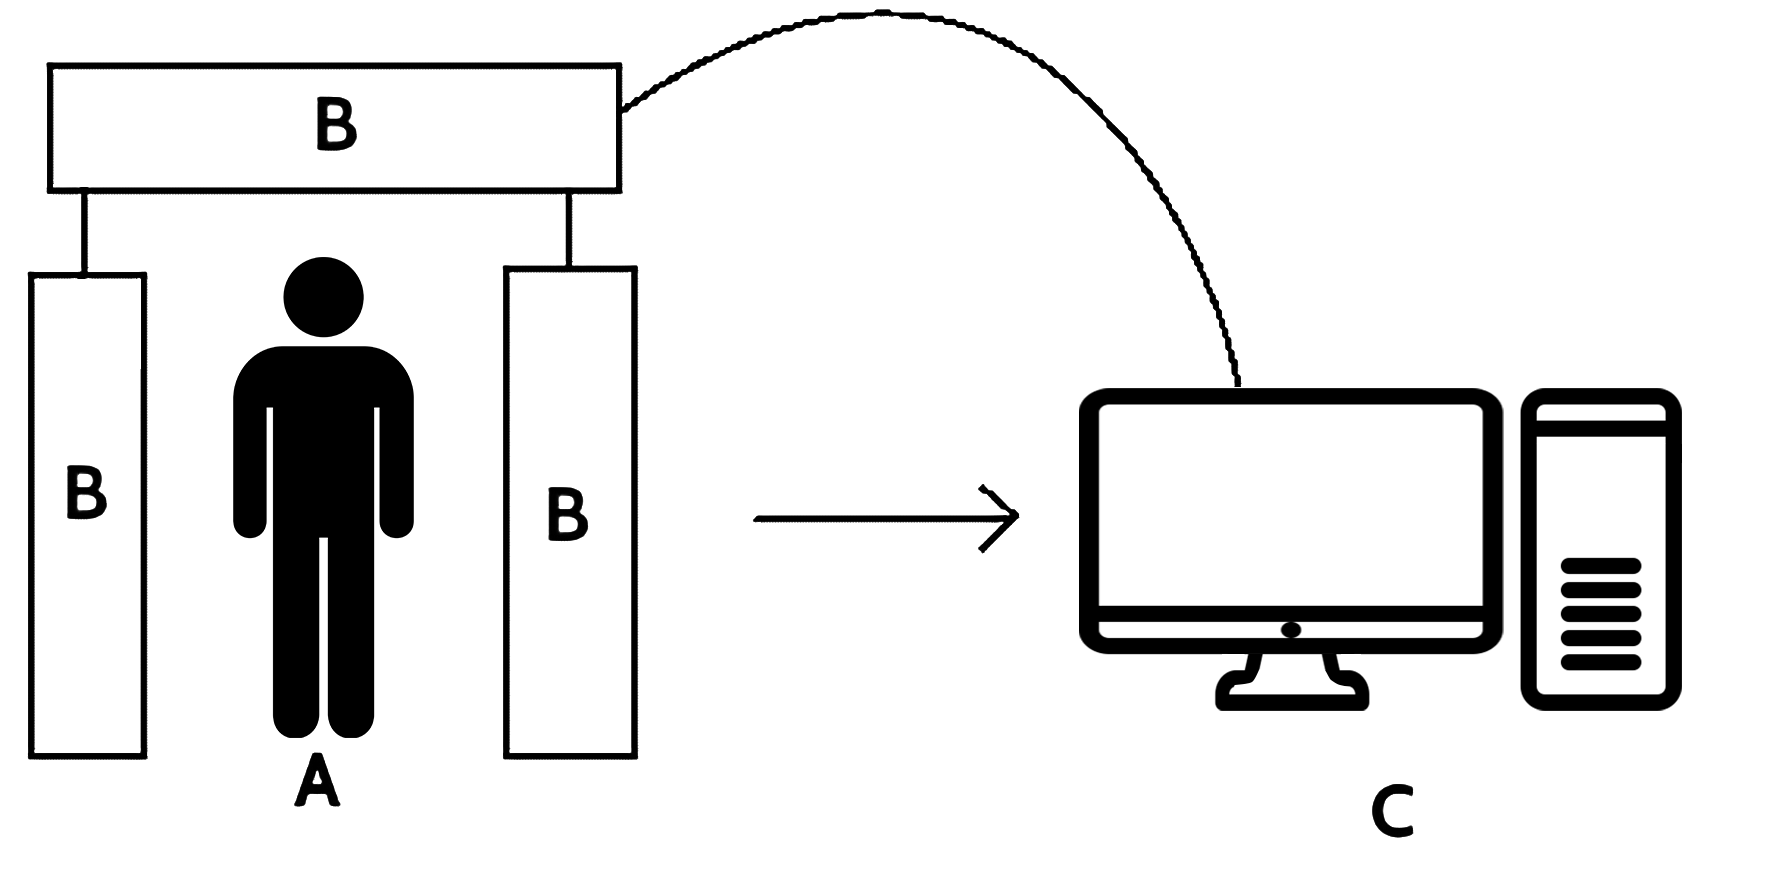
\includegraphics[width=0.8\textwidth]{kycia/BrainTransfer2.png}
 \caption{$A$---a human whose neural network is mapped by a device $B$. Using this mapping the model of the brain is constructed in $C$.}
 \label{Fig.BrainTransfer}
\end{figure}
%%%%
Assuming that the mapping by the machine $B$ can be undertaken accurately, the outcome $C$ is highly dependent on the nature of data $S$ stored in the brain of $A$. 

Three cases are as follows.


\textbf{Case 1---Brain data are stored in a classical physics structure.} In this case, a perfect copy of the data part of the brain can be made. The model of the brain---the copy--- can be made and no disruption to the original specimen $A$ (apart from the classical interaction of $A$ with measurement device $B$ which in principle can be done non-destructively) is made. As full information on the brain can be copied, the brain has no UA1 property. Besides, since in case of death or injury of the brain structures that store data disintegrate, therefore, no UA2 property is present. When the experiment of Fig. \ref{Fig.BrainTransfer} is performed, the two initially identical `brains' (the specimen $A$ and the copied model $C$) will operate at the same time independently.


\textbf{Case 2---Brain data are stored in quantum physics structures.} No copy of the brain can be performed without altering it and therefore the brain cannot be copied. As a result, this brain has the UA1 property. Moreover, as quantum data are non-destructible, according to Theorem \ref{Th.NoDeleting} the brain also has the UA2 attribute. If this assumption is valid, then the experiment from Fig. \ref{Fig.BrainTransfer} will result in transferring data (as no copy is permitted) to the model $C$ and therefore transcendence. The original brain $A$ due to the destructive nature of measurement during the transfer will be altered and cannot be considered as the initial $A$. Only one fully functional brain equivalent to the initial $A$ brain will operate at a given moment. A question arises as to the extent to which the functionality of $A$ will be altered. Given that the quantum component is essential for consciousness, the `copy' operation changes the state $A$ and therefore potentially creates a `philosophical zombie'.


\textbf{Case 3---Brain data contains both classical and quantum information.} This case is a mixture of both the above cases. The classical part of the brain data can be copied and destroyed and therefore the brain cannot have UA1 and UA2 properties. However, the quantum part of the brain data possesses these two properties. The experiment of Fig. \ref{Fig.BrainTransfer} will transfer the quantum part to $C$ and alter it in $A$; moreover, it will copy the classical part of the brain to $C$. Thus, the specimen $A$ will not be the same as before the transfer due to altering the quantum part transferred to $C$. As a result, only one fully functional model of the brain equivalent to the initial state of $A$ will be present at a given time. The second brain (in $A$) will be altered due to the measurement of quantum data transferred to $C$. If the quantum component is essential for consciousness, then its alteration in $A$ during the copying process may lead to a `philosophical zombie'. However, if the quantum component is irrelevant for consciousness, then the copy can be sufficiently accurate to make it impossible to distinguish the copy $C$ and the original $A$.

%%%%
\begin{figure}
\centering
 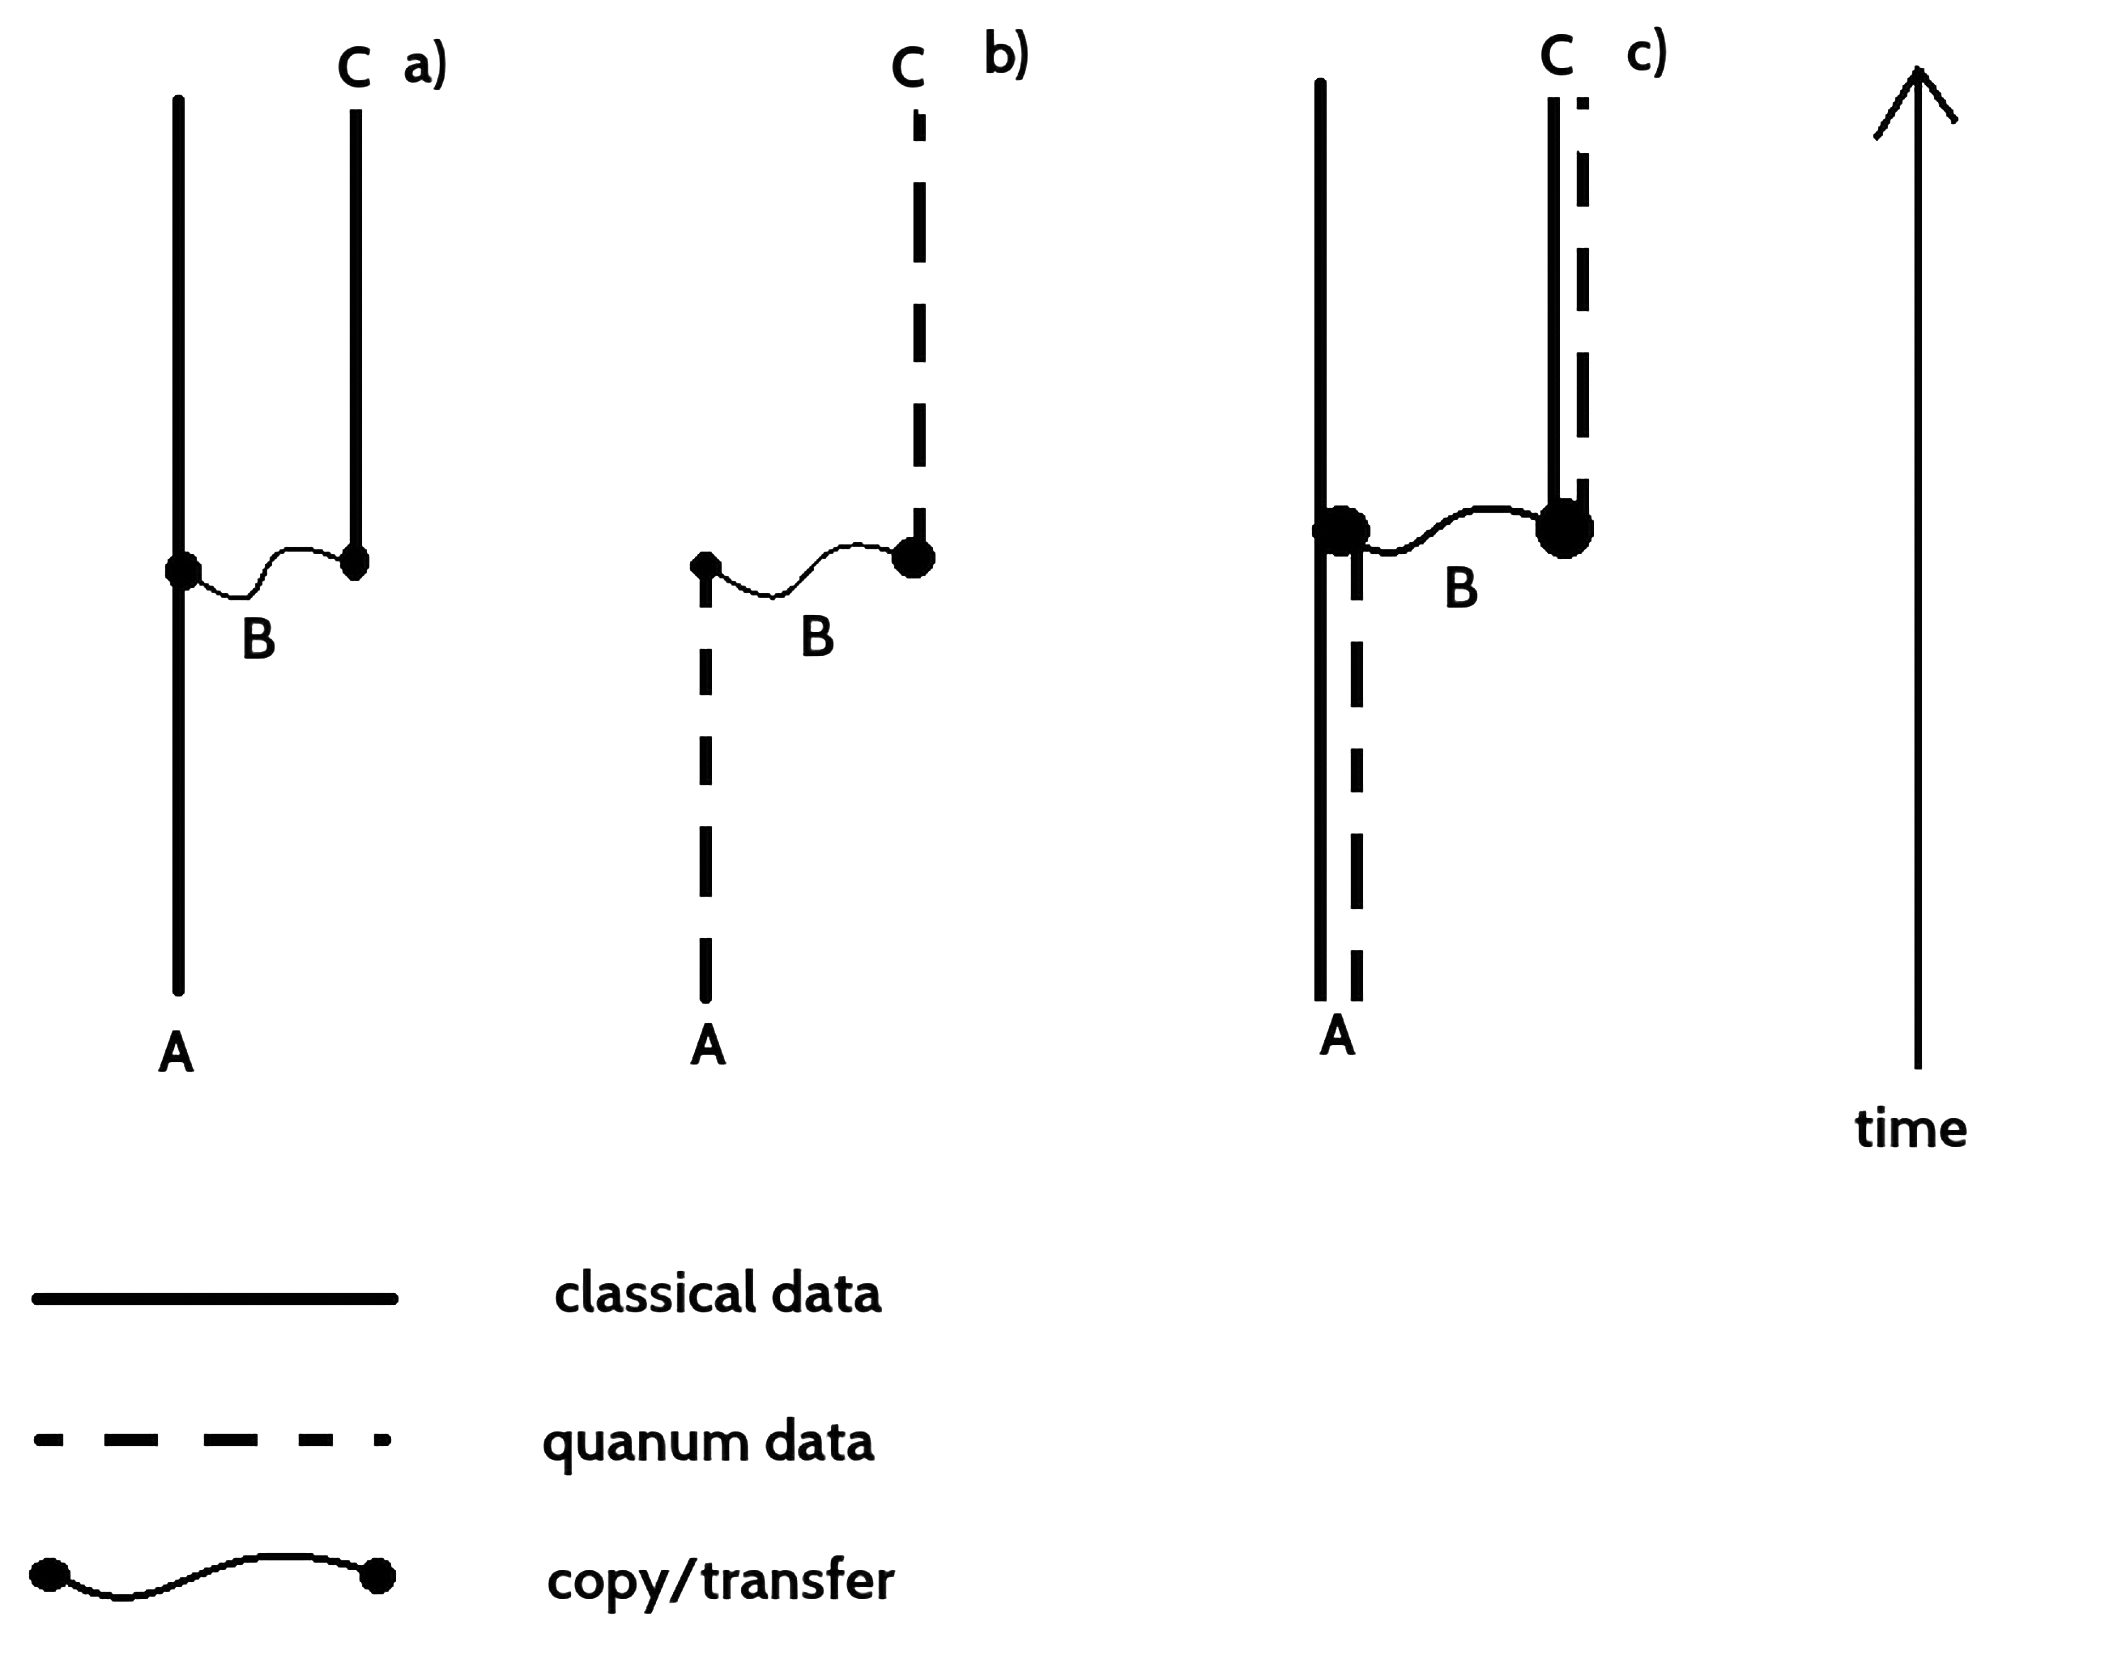
\includegraphics[width=0.7\textwidth]{kycia/TimeDiagram2.png}
 \caption{Case 1---a), Case 2---b) and Case 3---c) in time diagram. $A$- human, $B$- action of copy/transfer machine, $C$---simulator. One can observe that the quantum information is transfered and classical data copied. Quantum transfer alter original state.}
 \label{Fig.TimeDiagram}
\end{figure}
%%%%
These cases are presented in the time domain in Fig. \ref{Fig.TimeDiagram}.


For quantum data in the brain, one can perform copy with destruction, namely by measuring the quantum state of the brain (thereby altering this quantum state) and then creating a copy and restoring the brain's original state. In such a process, there is no continuity of existence of the original quantum state of the brain. However, there is a question as to whether it will be possible to set an altered brain quantum state $A$ to the original value before measurement. This depends on the complexity of the operation and the technology available. If the brain after quantum measurement can be set to the state before computation, then all quantum cases will have the same behaviour as in the classical case. 


As a conclusion from these cases, if the brain contains data that are quantum in nature, then it has properties UA1 and UA2.


The final subsection will present some remarks about the implications for metaphysical concepts.

%%%%%%%
\subsection{3.4. Metaphysical considerations}
%%%%%%%

The property UA1 (unable to be copied and therefore unique) does not imply indestructibility, defined by UA2. However, in the quantum case, both properties are present. Moreover, by UA2 property and by Theorem \ref{Th.NoDeleting}, the quantum state of the brain resides in the environment state after deletion and can be restored from it. If we assume that death is a quantum unitary deletion process, then the property UA2 describes some quantity that is preserved beyond the ceasing of the brain's computational functionality. We have attributed this to some part of the consciousness. However, the term `soul' \parencite{Soul}, which has additional metaphysical connotations, is more accurate for this property. In this context, the environmental state is the storage for `souls' attributed to the `afterlife'.

In this presentation, we have used the terms `soul' and `afterlife' without any religious connotations: they are the brain's quantum and environmental states, respectively. However, there is some similarity with the concept of soul (the immortal part of a human) and the afterlife. 


If the brain operates solely on classical principles (or if the quantum component is irrelevant), then `consciousness' is the proper term to use. In this case, the metaphysical part attributed to the `soul' must be regarded as an additional property, if one exists. 





%%%%%%%%%%%%%%%%%%%%%%%%%%%%%%%%%%%%%%%%%%%%%%%%%%%%%%%%%%%%%%%%%%%%%%%%%%%%
\section{Conclusions}
%%%%%%%%%%%%%%%%%%%%%%%%%%%%%%%%%%%%%%%%%%%%%%%%%%%%%%%%%%%%%%%%%%%%%%%%%%%%
Under reasonable assumptions as to the computational brain model and by employing properties of classical and quantum information, the possibility of performing the brain copy has been investigated. Only quantum properties result in the existence of a part of the brain that cannot be copied (and is therefore unique) and that cannot be destroyed. In the process, this investigation has explained the possible outputs of hypothetical brain copy experiments.


%%%%%%%%%%%%%%%%%%%%%%%%%%%%%%%%%%%%%%%%%%%%%%%%%%%%%%%%%%%%%%%%%%%%%%%%%%%
%Acknowledgments
%%%%%%%%%%%%%%%%%%%%%%%%%%%%%%%%%%%%%%%%%%%%%%%%%%%%%%%%%%%%%%%%%%%%%%%%%%%
\paragraph{Acknowledgments}

The author would like to thank Jacek Turnau for constructive feedback. The comments of Referees also made the paper clearer.

This research was supported by the GACR grant GA19-06357S, the grant 8J20DE004 of the Ministry of Education, Youth and Sports of the CR, and Masaryk University grant MUNI/A/0885/2019. RK also thanks the SyMat COST Action (CA18223) for partial support.



\paragraph{Author's statement}
All speculations in the paper are only the author's statements and do not reflect the viewpoint of any institution and should not be associated with them. All presented statements are logical conclusions from the available scientific results and imposed assumptions. The paper is written in a good will and by preserving the highest scientific standards. This paper is not intended to offend anyone. It is written as an attempt to describe the still yet unformalized area of human activity.

\end{artengenv}
\label{kycia_ende}



